The term classical computing in this document refers to Von-Neumann serial machines. This approach has brought modern day wonders like personal computers that ease the tasks like writing a novel, calculate incomes and expenses, watch films or talk to relatives living far away. 

As central processing units (CPUs) achieve higher clock frequencies their power consumption increases as well. This is commonly mitigated because newer generations are usually manufactured using smaller transistors, and since they need less power to operate the whole processor consumes less energy. The technology to manufacture such machines is now reaching physical limits and performance is not increasing as expected. One solution to this is to pack multiple processing cores in a single computing unit and run tasks in parallel, which has alleviated the performance hunger for the time being (Figure~\ref{fig:comp:moore}). 

\begin{figure}[h]
  \begin{center}
    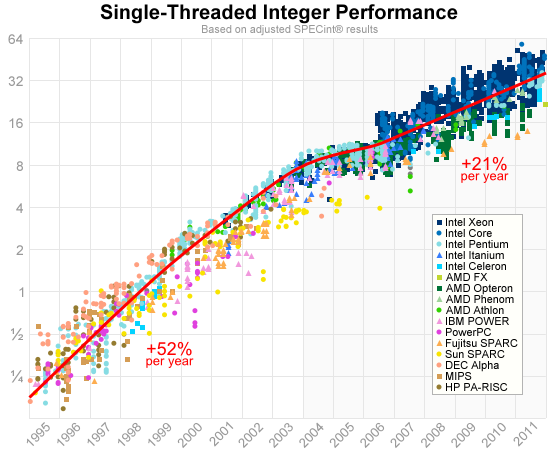
\includegraphics[width=0.7\textwidth]{integer-perf}
    \caption{Performance of CPUs vs release year, a steady increase is observed until about 2004, after that computing platforms where almost forced to use parallel processing~\cite{int-perf-images}. }
    \label{fig:comp:moore}
  \end{center}
\end{figure}

Even though classic CPUs have tremendous computing power, they have not been able to perform well on tasks that humans do without noticing (e.g. pattern recognition, inference, puzzles). This has lead computer manufacturers to design specialized processors to increase performance for specific tasks. A particularly successful example of this are 3D graphics accelerating cards, also known as Graphic Processing Units (GPUs), that model the graphics pipeline. They use multiple parallel processing units to calculate, which are a great match to the parallel nature of graphics computations~\cite{nickolls2010gpu,chen2009gpu}. Lately, general processing has been made possible in these cards though commercial applications other than graphics are just starting to emerge. Although GPUs are now considered highly parallel computing platforms and could be seen as a natural fit for neural networks, the data communication strategies are of a different nature and GPUs consume large amounts of power (high performance cards are rated at $>$ 300 watts )~\cite{nvidia, amd}.


